    \chapter{Experimental Design}
    \label{ch:experiment}
    \thispagestyle{fancy}
    
    The experiment was programmed using oTree \citep{chen2016}, and was conducted in four sessions at the \textit{Vienna Center for Experimental Economics} where a total of 96 people (55 female and 41 male) with an average age of 25 took part. Two of the sessions ran the control while the two others ran the treatment, such that exactly half the participants were in the treatment and half in the control.\\
    
    Participants were not allowed to communicate, nor to use their cellphones. The instructions were presented to all participants on-screen and were also read aloud to let them know everyone had the same information. Also, at every step during the instruction reading, participants were actively asked if they had any questions and we only proceeded if no one had.\\
    
    At the end of the session, participants were paid anonymously, in private, and in cash, ranging from EUR 12.5 to 31.3 for an average payoff of EUR 22.9.
    
    \section{General Structure of the Experiment}
    
    The experiment is roughly divided into three sections. The first is an introductory section where the Real Effort Task (RET), the leisure mode, the investment and prize awarding procedure, and, in the treatment, the taxation and redistribution scheme are explained in great detail. In this first section, participants are also asked several control questions to test for their understanding of the task.\\
    
    Within this introductory section, participants complete two rounds of the RET, once with a low piece rate and once with a high piece rate. This is used later as a baseline against which the performances in the competitive rounds are compared.\\
    
    The second section is the Tullock competition and it is the core of the experiment. In it, participants earn money by solving the RET which they can subsequently invest to win a higher piece rate in the following round.\\
    
    Finally, in the third section participants answer several questionnaires regarding their demographics, their cognitive reflection and their risk aversion.\\
    
    Figure \ref{fig:exp_str} shows the basic structure of the experiment, while table \ref{tab:exp_design} in the appendix lists a detailed breakup of the three main sections and its contents. The following sections in this chapter explain each part in detail.
    
\begin{figure}
\centering
\begin{tikzpicture}
  [
    grow                    = right,
    level distance          = 8em,
    edge from parent/.style = {draw, -latex},
    every node/.style       = {font=\footnotesize}
  ]
  \node(0) [root] {Instructions \&\\ Benchmark}
    child {node [env](ret) {RET}
                child{node[env]{Investment}
                    child{node[env](award){Award}
                        child{node[env]{Demographics \& \\ Control}
                    }
                }
            }
        };
      
      
    %draw the arrow from award to RET
    \draw[->]  (award) -- node {} ++(0,1cm) -| 
        (ret) node[pos=0.25, above] {High/Low Wage(8x)} 
        node[pos=0.75] {};
    
    
\end{tikzpicture}

\caption{Basic Structure of Experiment}
\label{fig:exp_str}
\end{figure}
    
    \section{Introductory Section}
    
    The introductory section welcomes the participants and instructs them into the functioning of the experiment and the Real Effort Task (RET).
    
    \subsection{Real Effort Task Instructions and Trial Round}
    
    After a short introduction to the experiment, participants are explained the main goal of the RET (counting "a"s) and how the submission works (typing the correct number in the input field and hitting "enter"). They then have the opportunity to test the task five times with five different sequences that were chosen to show the variability of the sequences. Some were long and some were short, some had many and some had few "a"s. (an in-depth explanation of the RET is presented in section \ref{ss:RET}) \\
    
    The screen also featured an annotated tour that explained every part of the RET screen: the sequence, the input field, and a timer counting the number of seconds needed to solve the current and the previous sequence.\\
    
    When a correct answer is submitted, the next sequence is shown and the current timer is restarted.
    
    \subsection{Switch Mode Instructions}
    
    After participants have completed the trial round, they are introduced to the leisure mode, the payment scheme, and the increasing difficulty mechanism of the RET. The incentivised leisure mode is a core feature of my experiment and it is explained in more detail in section \ref{ss:RET}. During the experiment it is called "switch mode" to avoid any stigma on shirking.\\
    
    Participants are paid one token per correctly solved sequence with one token being converted to \EUR{0.1} at the end of the session. While in the "switch" mode, they earn 0.1 tokens per each second spent in it. Great effort is put in this screen to let participants know that, given the payoffs, the ideal point to switch is when he or she takes longer than 10 seconds to solve a sequence, regardless of how much time is left or how many sequences they have solved thus far. However, I do not explicitly write that as an optimum since in the competition rounds it might be advisable to solve more sequences to increase the chances of a higher piece-rate.\\
    
    In this screen, an illustrative example of possible earnings is presented, participants can test the RET several times, and an annotated tour introduces the new elements (a counter of total solved sequences a timeout, and the switch button).
    
    \subsection{Control Questions}
    
    In this page, participants are asked two sets of questions to ensure that they have understood the instructions. To be able to proceed, they have to answer all questions correctly.\\
    In the first set, participants are asked how much a fictional player would have earned given an amount of solved sequences and time spent in the "switch" mode (fig. \ref{fig:cq_earnings}). The numbers were chosen so they would not offer an obvious anchor point\footnote{An anchor point being an amount of time or sequences solved that a participant is supposed to aim to while solving the RET} while still being easy to calculate.
    
    \begin{figure}
        \centering
        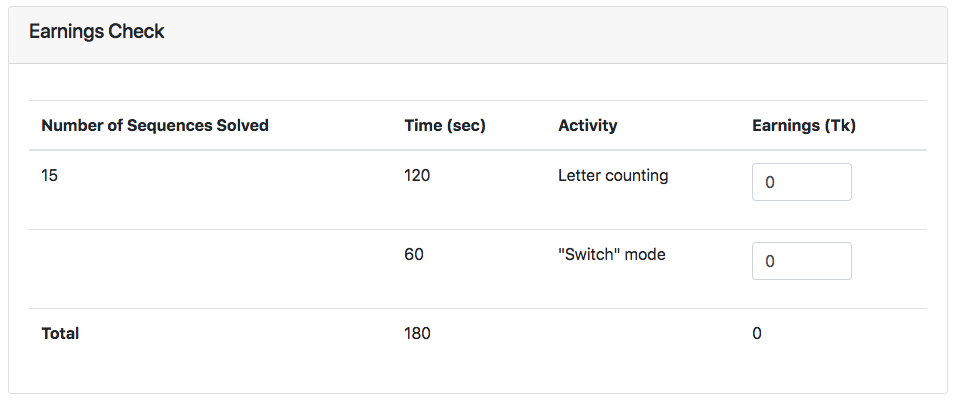
\includegraphics[width=\textwidth]{graphs/cq_earnings.png}
        \caption{Control Question Earnings}
        \label{fig:cq_earnings}
    \end{figure}
    
    In the second set (fig. \ref{fig:cq_switch}) participants were asked to select the switching point of a fictional player aiming at maximizing her payoff. Also here the times were selected in such a form, that a tendency to infer an anchoring point would be minimized. Similarly, instead of giving examples of actual sequences, only a visualization with bars is given.
    
    \begin{figure}
        \centering
        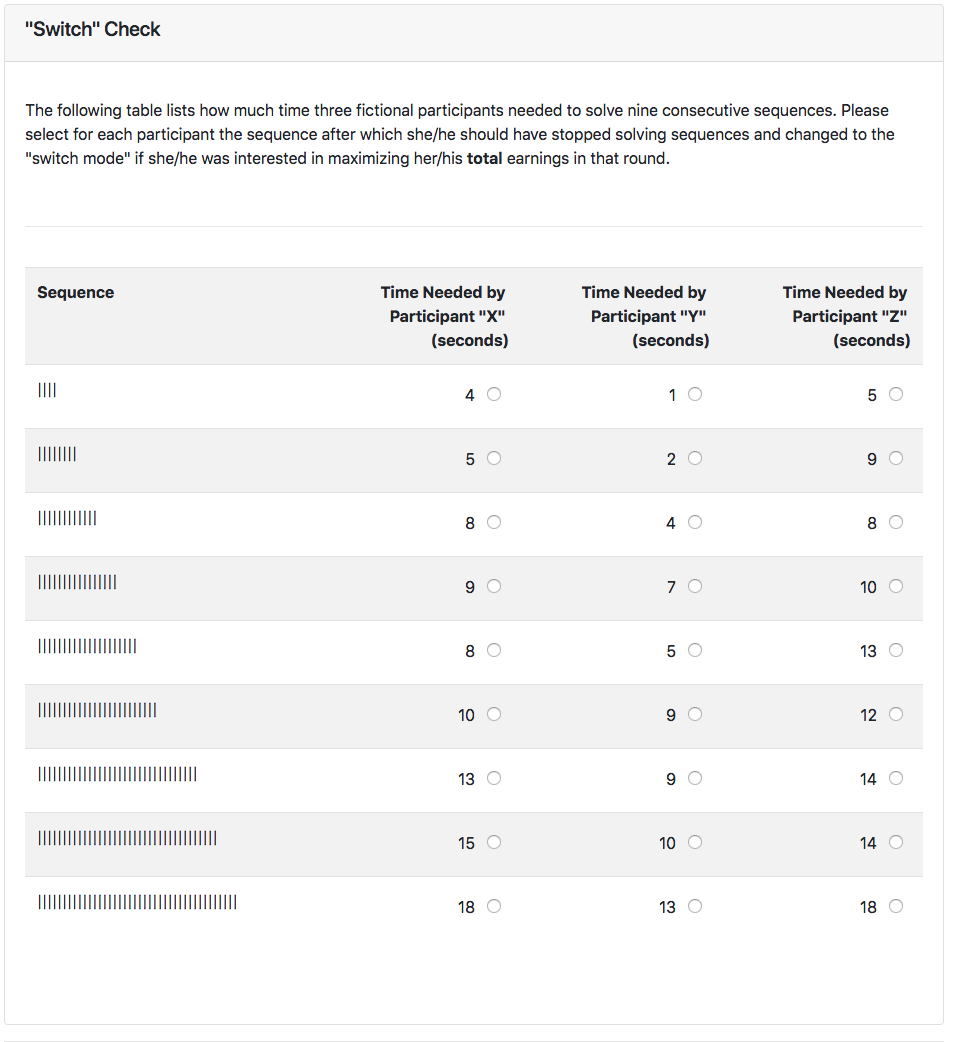
\includegraphics[width=\textwidth]{graphs/cq_switch.png}
        \caption{Control Question "Switch" Mode}
        \label{fig:cq_switch}
    \end{figure}
    
    
    \section{Real Effort Task}
    \label{ss:RET}
    
    Every time, before the Real Effort Task (RET) starts, a waiting page makes sure that all participants have completed all sections before, thus avoiding some participants solving the task while others read. Also, a confirmation page is displayed before the RET so that participants are ready when it starts.\\
    
    The RET is inspired by \cite{rey-biel2016} and \cite{giusti2014}. Participants are asked to count the occurrences of the letter "a" in a random string of characters. Figure \ref{fig:LC_screen} gives an example of such a string which in the experiment is called a \textit{sequence}. The sequence is generated pseudo-randomly but it is identical for every participant in the session. A fact that all participants are made aware of.\\ 
    
    \begin{figure}
        \centering
        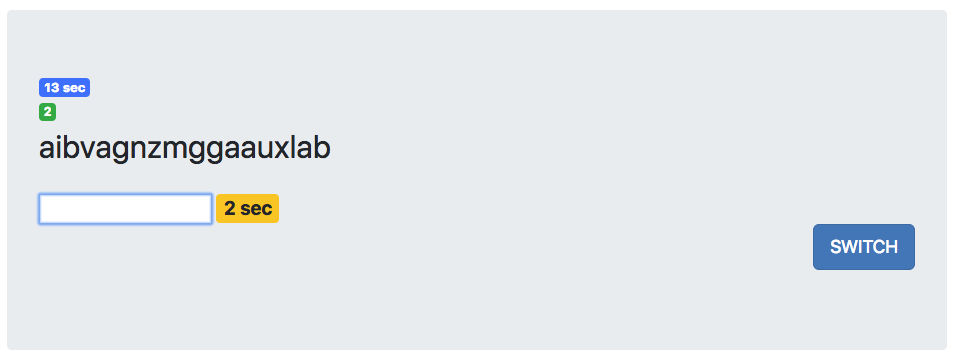
\includegraphics[width=\textwidth]{graphs/screenshot_RET_alone.png}
        \caption{Sample Screen of the Letter Counting Task}
        \label{fig:LC_screen}
    \end{figure}
    
    This particular task has been chosen as it fulfills several requirements from my design. The main research questions address the effects of inequality on performative measures like output, and efficiency. To be able to observe changes in those measures it is therefore important to ensure that participants are not simply always doing as much as they can, i.e. a corner solution. Such a phenomenon would be particularly strong if players have a strong intrinsic motivation or if no incentive is offered to stop solving tasks \citep{frey1997}. An example of a task with high intrinsic motivation would be any fun game like, for instance, Tetris.
    The Letter Counting Task is tedious and repetitive without being effortless and therefore offers a particularly strong effect for monetary incentives \citep{cerasoli2014}.\\ 
    
    Furthermore, the task is easy to explain and it does not rely on a mathematical framing which has been shown to induce a gender gap, when in a competitive setting, not linked to skill \citep{niederle2010}.\\
    
    Several other mechanisms that are explained later further ensure that players do not stay in the game only to avoid boredom and that, given a player's ability, an optimal work supply level exists.
    
    \subsection{Learning Effects}
    Since the experiment consists of several benchmarking and competition rounds it was important to have a task that would present little increase in performance after each repetition. Otherwise it would have been difficult to compare the outcomes of the baseline and the competition rounds for the same participants.\\
    
    The task and design selected allow for enough repetition and learning even before starting. Furthermore, within each round there are several repetitions. In average, a participant solves 11.6 sequences per round. There does not seem to be much room for improvement in recognizing "a"s after doing it a couple times. Figure \ref{fig:exp_str} shows the average time needed to solve the first 16 task across the eight competitive rounds. Although there is an increase in variance as the task become more difficult (going from the top left to the bottom right box), there is no visible decrease in the average time needed by participants to solve each task across rounds (going from left to right in each box). Furthermore, I assume similar learning effects across individuals.
    
    \begin{figure}[h]
        \centering
        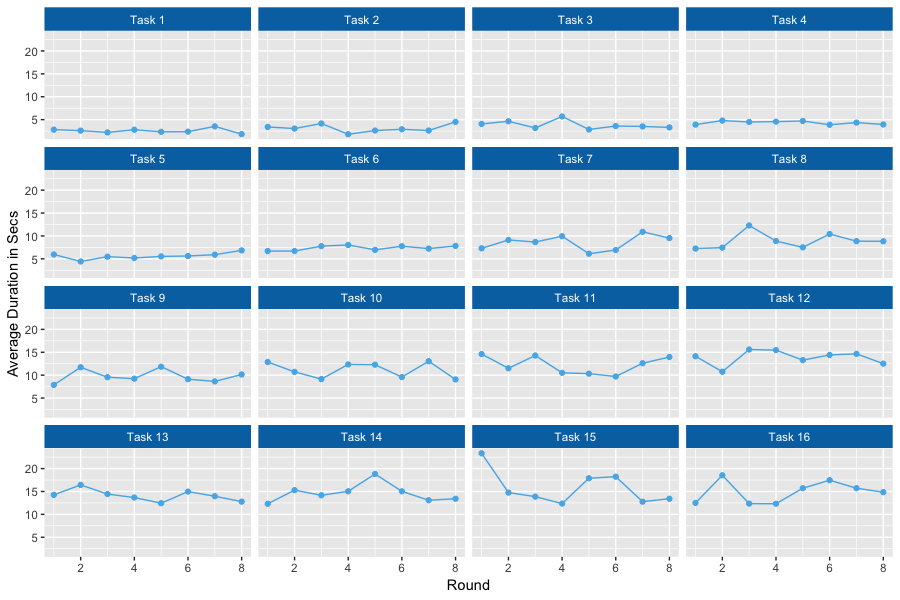
\includegraphics[width=\textwidth]{graphs/avg_time_per_task_round.png}
        \caption{Average time in seconds needed to solve the first 16 tasks across rounds}
        \label{fig:avg_time_task}
    \end{figure}
    
    \subsection{Incentivised Leisure}
    
    As already mentioned above, another issue present when identifying levels of work supply is the missing of incentivisation of non-work. In real life, leisure has an intrinsic motivation which in economics is quantified by the opportunity costs of not working. In the laboratory, however, due to the short time frame, implicit peer presure and possible experimenter demand effects, participants might be averse to stop supplying work and spend time in leisure. To address this issue, a fundamental feature of my design is, following (sausgruber etal), the monetary incentivisation of leisure time.\\
    
    In my experiment, participants have, at any point while solving the task, the opportunity to change to a leisure mode where they are paid per time unit and do not need to work. This leisure time mode is called "switch" to avoid any stigma on shirking \citep{rey-biel2016, eriksson2009}. To ensure that participants do not enter the switch mode by mistake, a confirmation screen is shown.
    
    \subsection{Increasing Difficulty and Optimality}
    
    Given a participant's ability, there must exist a rate of payment per time unite for which she or he is indifferent between offering work -solving the task- or spending time in leisure. Assume for instance that a participant needs one second to solve a sequence of given length and earns one monetary unit for that. If he or she would also earn one monetary unit per second in the leisure mode, they would stay in the "switch" mode since there is also a disutility to labor. But if he or she needs shorter than one second, they would prefer to solve the sequence since they would earn more. Between those two points, and according to the transitivity and continuity axioms of choice, there must be a point where they were indifferent.\\
    
    In my design, and following ---sausgrubers-- idea, the Letter Counting Task starts at a level for which any participant would earn more by solving the task than by spending time in "switch" mode. The sequence then increases in length each time by four characters making it each time more difficult to count the number of "a"s. Depending on their abilities, each player will have a point at which he or she would earn more by staying in the "switch" mode. By observing the times taken to solve each task I can infer the point at which any participant should have changed.\\
    
    This difficulty increasing feature is also one of the reasons for which I chose the Letter Counting Task. The random sequence is easily generated while the difficulty increase (the length increase) can be easily and quantifiably changed. In fact, it allows for several parameter changes for future research. For instance the speed of increase, the exchange rate between "switch" and task, or the letters that are to be counted.\\
    
    To ensure that, when generated, the solution to the following sequence is not just the number of the last sequence plus a small number, for each generated sequence a new sample from a new population with a different distribution is drawn. This makes it unviable to just guess the number of the sequence by starting at the number of the last one.
    
    \subsection{Benchmarking}
    
    To identify the levels of performance outside competition, two rounds of the RET are played during the introductory section of the experiment. In the first round, the low piece rate is payed, while in the second the high piece rate is payed. The latter was, in my case, double the piece rate of the first round such that a participant would take up to twenty seconds solving a sequence before switching to the leisure mode. The low piece rate was selected first because I wanted to make the increase in earnings with the higher piece rate more salient.\\
    
    Instructions and control questions were shown before the high piece rate paying round. In the control questions, I chose the possible answers such that selecting the correct answer for the last round would be possible, so forcing participants to think why there was a change in the maximizing time to solve sequences.
    
    \subsection{Taxed Benchmarking}
    
    To better measure the valuation of the price in the taxation treatment, two extra rounds with a taxation equal to the effective rate in the treatment were introduced. Specifically, in between the low piece rate and high piece rate another round was introduced. This round payed per task the equivalent of the effective taxed low piece rate after redistribution or $w(1-t)+ w(t/3)$, in my case, 0.6 tokens per sequence. The payment for the \textit{switch} mode remained, as in all rounds, constant. Similarly, an extra round was introduced after the high wage round which payed the equivalent of the effective taxed high piece rate after redistribution, in our case, 1.2 tokens. This extra rounds were introduced in this order so as not to generate a strong separation between the taxed and the untaxed rounds, as well as to space out the control questions. \\ 
    
    A t-test analysis shows that there are no differences between the production in the high piece rounds, i.e., no learning or timing effects, nor were significant differences between the low piece rate rounds, i.e. no skill differences.
    
    \subsection{Feedback}
    
    During solving of the RET a summarized version of the instructions is shown at the bottom of the page and a mouseover display explains all relevant elements if needed. Once a participant goes into the "switch" mode, a counter shows live how many tokens he or she earns with each passing second and informs him or her about the number of sequences solved.\\
    
    Finally, a feedback screen shows how many sequences were solved, how much time spent in the "switch" mode and how many the total earnings for the round are. In the second round of the baseline setting RET, another table informs the participant about the earnings of the previous round to make the difference in earnings, between the high and the low piece rate, more salient.
    
    \section{Competition Section}
    \label{ss:compt}
    
    In this section, participants are informed that they were selected randomly into groups of three people and that each one was assigned a label \textit{A, B} or \textit{C}, but that their identity and that of all other participants will remain anonymous both to all other participants as well as to the experimenters\footnote{in order to reduce the impact of other-regarding behavior}. Participants in the treatment sessions are farther informed at this stage about the taxation and redistribution scheme (see section \ref{ss:treat}).\\
    
    Between the introductory section and the competition, two things change with the RET. One the competitive aspect of being in the group. In fact, last place aversion and the utility of winning itself are driving issues behind overbidding in rent-seeking contests \citep{sheremeta2013}. Second, the actual contest where increasing one's earnings can also indirectly increase the chances of winning the prize (trough a larger available income to invest).\\
    
    A possible workaround could have been to add two rounds without an investment or prize option. however, this could nevertheless have been used to send signals about the own valuation of the prize to other participants. Since a participant with a higher valuation would also invest more, sending signals about he own valuation might be rewarding even if no prize is to be immediately won. Since, as shown in section \ref{sec:budget_constraint}, the impact of the second aspect is not taken into account for the present thesis. 
    
    \subsection{Tullock Contest}
    
    Next, players are informed  about the contest itself. In eight rounds, each participant will have the opportunity to earn money by solving the letter counting task or spending time in the "switch" mode. Money earned by counting letters\footnote{or, in the treatment, the net income plus the redistributed amount} can then be invested to increase the higher piece rate in the following round. Only one person per round is awarded the prize and the probability of winning it is equal to the share of that person's investment relative to all investments by all players. An example for easier understanding is also shown.\\
    
    Players are farther reminded at this stage of their earnings in the introductory section and of the difference in earnings between the low and high piece rate rounds. This difference is what is interpreted as their valuation at the moment of judging their investments.
    
    \subsection{Beliefs}
    
    To test if and how much players take into account the behavior of the others when choosing their production and investment levels, beliefs about the production, i.e. the number of sequences solved, and the amount invested by the other team members are elicited in every round. A visual clue lets them know which player has a higher piece rate in the current round.
    
    \subsection{Feedback and Result}
    
    After solving the task and before investing, as in the introductory section, participants receive feedback on their performance: how many sequences were solved, how many seconds spent in "switch" and, in the case of the treatment, how much the transfers are.\\
    
    After the investment, participants become detailed feedback about the investments and performance of the group (see fig. \ref{fig:screen_results}).
    
    \begin{figure}
        \centering
        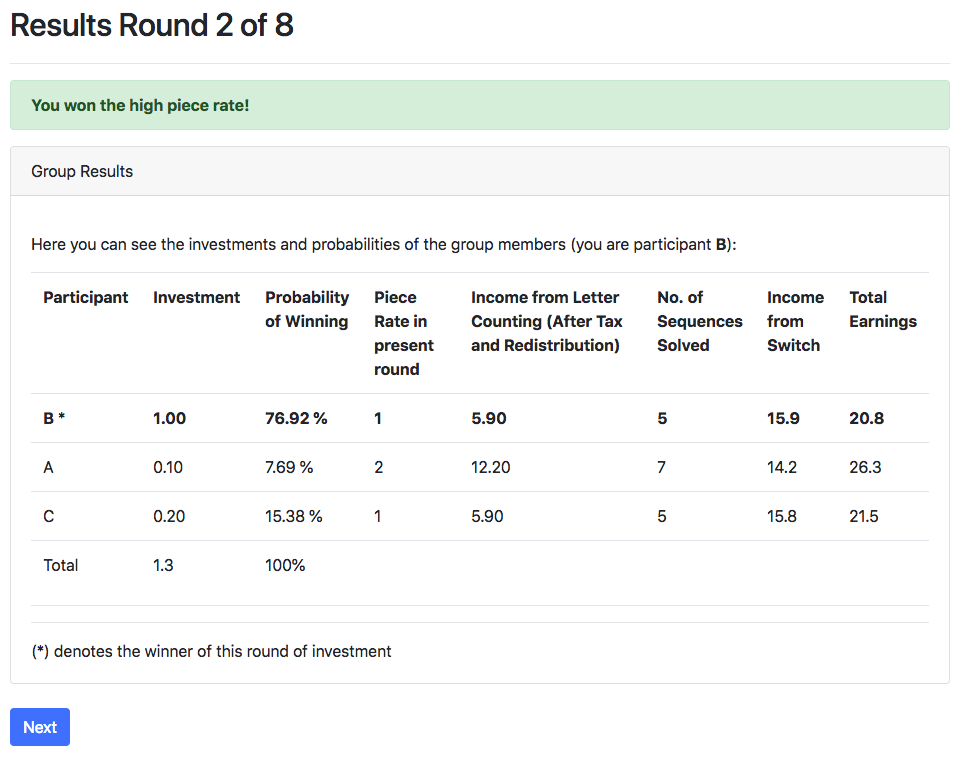
\includegraphics[width=\textwidth]{graphs/screen_results.png}
        \caption{Results Screen after Investment}
        \label{fig:screen_results}
    \end{figure}
    
    \subsection{Investment}
    
    In the investment screen, players use a slider to choose their investment in steps of 0.1 tokens. They are informed about their total available income for investment, how much they invest, how much they would keep and what the prize is. They are also recalled that tokens invested are not refunded, even if the prize is not awarded (see fig. \ref{fig:screen_invest}).
    
    \begin{figure}
        \centering
        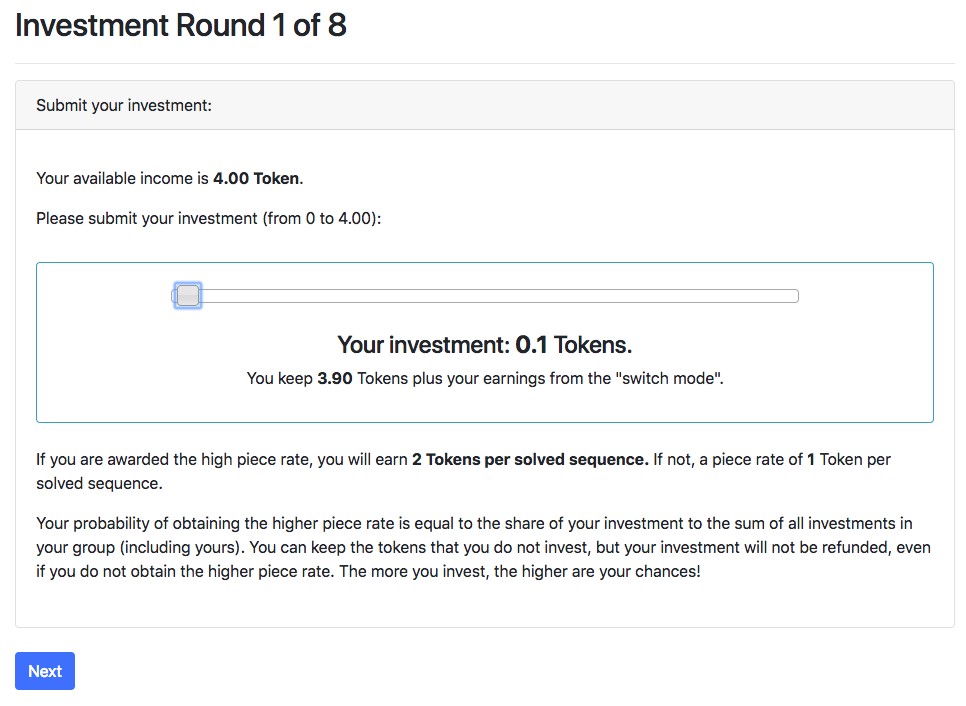
\includegraphics[width=\textwidth]{graphs/screen_invest.png}
        \caption{Investment Screen}
        \label{fig:screen_invest}
    \end{figure}
    
    
    \section{Treatment: Taxation and Redistribution of Income}
    \label{ss:treat}
    
    Income from work, that is, from counting letters, is taxed in the treatment at 60\%. The entire tax revenue is then divided equally among all participants so that the total amount of tokens in circulation is constant. Participants can then invest their net income plus transfer to increase their chances to earn the higher piece rate as explained in section \ref{ss:treat}.\\
    
    In the control group there is no taxation and therefore no redistribution. The available income to invest is exactly equal to the earned tokens from letter counting.
    
    
    \section{Risk Aversion Measure and Risk Elicitation}
    
    In the investment section of the experiment players participate, effectively, in a lottery. The exact terms of that lottery are not known to them in advance and present an strategic decision as well. Their investment choices will therefore not only reflect their strategic considerations, but also their stance on risk taking.\\
    
    To control for this I include an incentivised risk elicitation test following the \textit{Multiple Price List} by \cite{holt2002} (HL) with the implementation for \textit{oTree} taken from \cite{holzmeister2017}.\\
    
    I chose the HL method as it, according to \cite{crosetto2016} and \cite{harrison2008}, among other things:
    \begin{itemize}
        \item allows for risk preferences in both the risk neutral and risk seeking range
        \item has a finer categorisation as for instance \cite{eckel2008}
        \item has constant intervals between the parameters of risked mapped trough choices which makes it robust to stochastic decisions
        \item there are no significant differences between genders
    \end{itemize}  
       
     In the HL method, players are asked to choose between several pairs of lotteries, A and B. Beginning with a choice where option A is the safer choice, the last choice is between sure outcomes, where B represents the payoff maximizing choice. Between them, there is a point where a participant changes from one option to the other, thus revealing her risk preferences.\\
     Figure \ref{fig:choices_mpl} shows the list of choices that participants were presented with. In it, probabilities are visualized with the help of pie charts and all possible decisions are shown at once. Consistent preferences were forced to avoid elimination of data in the already small sample. After choosing, one of the decisions was then selected randomly and the lottery drawn and paid out.\\
     
     \begin{figure}
         \centering
         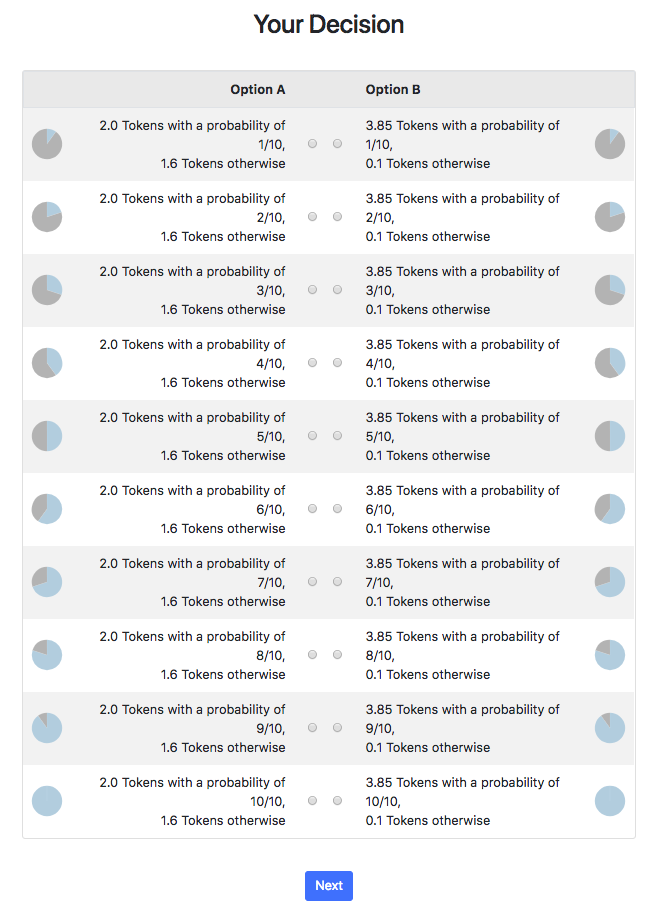
\includegraphics[width=\textwidth]{graphs/Choices_MPL.png}
         \caption{Choices Screen \textit{Multiple Price List}}
         \label{fig:choices_mpl}
     \end{figure}
     
     
    Following the common procedure I assume participants to have a constant relative risk aversion (CRRA) utility function $u(x)=x^{(1-r)}$, which allows to index each choice by a corresponding $r$. An individual with an $r<0$ is categorized as risk averse, with $r=0$ as risk neutral and with $r>1$ as risk seeking. The payoffs are exactly equivalent to those used by \cite{holt2002} and thus imply, that someone switching after the fourth lottery to \textit{option B} is assigned an $r$ interval of (-0.15, 0.15) meaning risk neutrality. The list of the implied risk aversion ranges can be seen on table \ref{table:HL} where the number of safe choices is the number of choices before switching to \textit{option B}.
    
    
    \begin{table}[]
    \centering
    \begin{tabular}{lll}
    \hline
    \hline
    \begin{tabular}[c]{@{}l@{}}Number of \\ Safe Choices\end{tabular} & \begin{tabular}[c]{@{}l@{}}Range of Relative\\ Risk Aversion\end{tabular} & \begin{tabular}[c]{@{}l@{}}Risk Preference \\ Classification\end{tabular} \\
    \hline
    0-1                                                               & r < -0.95                                                                 & Highly Risk Loving                                                        \\
    2                                                                 & -0.95 < r < -0.49                                                         & Very Risk Loving                                                          \\
    3                                                                 & -0.49 < r < -0.15                                                         & Risk Loving                                                               \\
    4                                                                 & -0.15 < r < 0.15                                                          & Risk Neutral                                                              \\
    5                                                                 & 0.15 < r < 0.41                                                           & Slightly Risk Averse                                                      \\
    6                                                                 & 0.41 < r < 0.68                                                           & Risk Averse                                                               \\
    7                                                                 & 0.41 < r < 0.97                                                           & Very Risk Averse                                                          \\
    8                                                                 & 0.41 < r < 1.37                                                           & Highly Risk Averse                                                        \\
    9-10                                                              & 1.37 < r                                                                  & Stay in Bed\\
    \hline
    \end{tabular}
    \caption{Risk Aversion Classifications Based on Lottery Choices\\ \citep{holt2002}}
    \label{table:HL}
    \end{table}
    
    \section{Cognitive Reflection Test}
    
    A tendency to overbidding in rent-seeking contest has been well documented \citep{sheremeta2013, dechenaux2015}. This is particularly critical in my design as overbidding, both in terms of work supply and investment, would be interpreted as an over-exertion of effort.\\
     
    While there are several proposals as to what influences this behavior, \cite{sheremeta2016} suggests that impulsiveness might be the strongest predictor. In fact, he suggests that when analyzed simultaneously with the utility of winning, systematic biases, relative payoff maximization, and mistakes, only impulsiveness remain statistically significant.\\
    
    Following him I therefore include a \textit{Cognitive Reflection Test} based on \cite{thomson2016}. The latter propose alternative questions that also measure cognitive reflection but are less well known. Figure \ref{fig:crt_quest} shows the questions that participants were presented. although they were presented singularly, instead of all at once.
    
    \begin{figure}
        \centering
        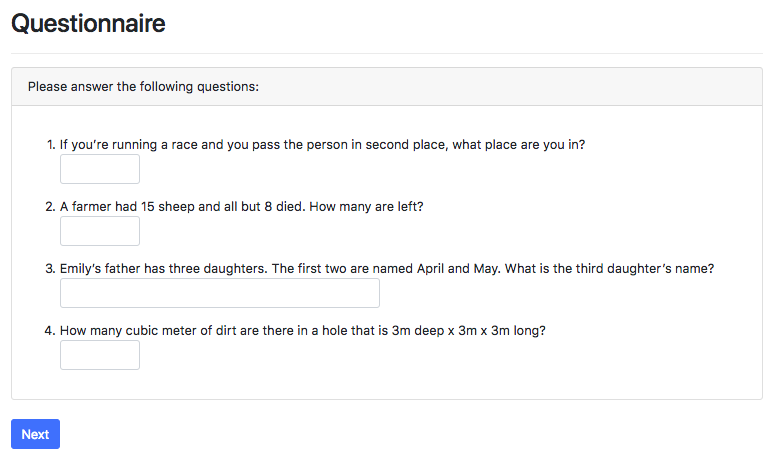
\includegraphics[width=\textwidth]{graphs/CRT_Quest.png}
        \caption{Cognitive Reflection Test \citep{thomson2016}}
        \label{fig:crt_quest}
    \end{figure}
    
    \section{Hypotheses}\label{ss:hyp}
    
     \begin{hyp} \label{hyp:treat}\textit{The mean difference in Probability of Upward Mobility between high and low earners will be decreased in the taxation treatment}\end{hyp}
     
     
     
      
      An important corollary of \cref{hyp:treat} is that, since players are closer to the optimum levels of both work supply and investment, total welfare for the group in terms of total income generated is larger.\\
      
        To test this hypothesis both groups are compared in each round using a mixed ANOVA design. Dependant variables are the number of seconds spent over the optimum (10 or 20 depending on piece rate) by the group, the share of investment to valuation and total generated income before and after investment.
        
    
    \begin{hyp}\label{hyp:wins}
    \textit{A participant who won the first round of the Tullock Contest will be more likely to have more wins in the control than in the treatment, even after controlling for skill, risk aversion and crt.}
    \end{hyp}    
    
    
    \begin{hyp}\label{hyp:a} Participants in groups with higher inequality will invest less relatively to their valuation and spend more time in leisure.\end{hyp}
    
    To test this hypothesis I determine the inequality level before investment, investment level, and production level of each group and run a panel analysis.
    
    
    
